\documentclass{article} 
%%
%% This document template assumes you will use pdflatex.  If you are using
%% latex and dvipdfm to translate to pdf, insert dvipdfm into the options.
%%

%%%%
%% Package includes to provide the basic style
%%
\usepackage{harvard}    % Uses harvard style referencing
\usepackage{graphicx}   % Permits import of various graphics formats
\usepackage{hyperref}   % Provides hyperlinks to sections automatically
\usepackage{pdflscape}  % Provides landscape mode for end code listings
\usepackage{multicol}   % Provides ability to split output into columns
\usepackage{listings}   % Provides styled code listings


%%
%% Set some page size changes from the standard article class
%%
\usepackage{calc}
\setlength{\parskip}{6pt}
\setlength{\parindent}{0pt}
\addtolength{\hoffset}{-0.5cm}
\addtolength{\textwidth}{2.5cm}


%%
%% Format definitions for the style
%%
\bibliographystyle{agsm}  %{alpha}
\citationstyle{dcu}
\pagestyle{headings}
\fussy


%%
%% Definitions to provide layout in the dissertation title pages
%%
\newenvironment{spaced}[1]
  {\begin{minipage}[c]{\textwidth}\vspace{#1}}
  {\end{minipage}}


\newenvironment{centrespaced}[2]
  {\begin{center}\begin{minipage}[c]{#1}\vspace{#2}}
  {\end{minipage}\end{center}}


\newcommand{\declaration}[2]{
  \thispagestyle{empty}
  \begin{spaced}{4em}
    \begin{center}
      \LARGE\textbf{#1}
    \end{center}
  \end{spaced}
  \begin{spaced}{3em}
    \begin{center}
      Submitted by: #2
    \end{center}
  \end{spaced}
  \begin{spaced}{5em}
    \section*{COPYRIGHT}

    Attention is drawn to the fact that copyright of this dissertation rests
    with its author. The Intellectual Property Rights of the products
    produced as part of the project belong to the author unless otherwise specified
    below, in accordance with the University of Bath's policy on intellectual property 
   (see http://www.bath.ac.uk/ordinances/22.pdf).

    This copy of the dissertation has been supplied on condition that anyone
    who consults it is understood to recognise that its copyright rests with its
    author and that no quotation from the dissertation and no information
    derived from it may be published without the prior written consent of
    the author.

    \section*{Declaration}
    This dissertation is submitted to the University of Bath in accordance
    with the requirements of the degree of Bachelor of Science in the
    Department of Computer Science. No portion of the work in this dissertation
    has been submitted in support of an application for any other degree
    or qualification of this or any other university or institution of learning.
    Except where specifically acknowledged, it is the work of the author.
  \end{spaced}

  \begin{spaced}{5em}
    Signed:
  \end{spaced}
  }


\newcommand{\consultation}[1]{%
\thispagestyle{empty}
\begin{centrespaced}{0.8\textwidth}{0.4\textheight}
\ifnum #1 = 0
This dissertation may be made available for consultation within the
University Library and may be photocopied or lent to other libraries
for the purposes of consultation.
\else
This dissertation may not be consulted, photocopied or lent to other
libraries without the permission of the author for #1 
\ifnum #1 = 1
year
\else
years
\fi
from the date of submission of the dissertation.
\fi
\vspace{4em}

Signed:
\end{centrespaced}
}

%%
%% END OF DEFINITIONS
%%

    %% These are the includes required for the doc 

\usepackage{scrextend}
\usepackage{graphicx}



\title{Ghoul Hunter, an augmented reality location based mobile game whose game objects are generated using a statistical model that ensures game balance}
\author{Harry Martin}
\date{Bachelor of Science in Computer Science with Honours\\The University of Bath\\October 2016}

\setlength{\parindent}{0pt}
\newcommand{\forceindent}{\leavevmode{\parindent=1em\indent}}


\begin{document}
	\bibliographystyle{plain}
	\maketitle
	
	\section{Problem Description}
	\paragraph{}Augmented reality mobile games are a relatively new type of gaming that has become very popular since the launch of Pokemon GO \cite{pokemon_go}. Augmented reality games enhance the real world with generated game objects.  Typically these games tie game objects to geographical locations. The player can then interact with game objects by going to there location. Once they are near the location of a game object the player can see a graphical representation of the game object over the top of the phone's camera image. The generation of game object must keep the game balanced. Not too many of one game object and not too few of other. A correct balance of game objects will maximise enjoyment of the game by correctly determining the reward to effort ratio. 
	
	\paragraph{}Most augmented reality games do not restrict game objects locations to the game object's type. The closest game to doing this is Pokemon GO which is more likely to generate pokemon in certain areas based on the pokemon's type. For example water pokemon are more likely to generate near rivers or lakes. However no popular augmented reality game has completely restricted the generation of game objects to certain geographical locations. For example wood only being generated in forests. This creates new problems when generating game objects. The task of balancing the game is a little more complex as different areas of the map will have different amounts of forests, roads, buildings and so on. A generation algorithm would have to take this into account while trying to generate an appropriate amount of game object's for each area of a map. 
	
	\paragraph{}No popular augmented reality mobile game has used the concept of resources. Resources are atomic game objects that the player can collect to transform into other game objects. This makes the concept of game balance especially important as resource generation will determine how easy other game objects are to build. If resources are too plentiful then it will take little effort to create valuable game objects but if resources are too few then relatively basic game objects will be too difficult to obtain. 
	
	\paragraph{}Furthermore augmented reality games have not fully explored the potential of real time battles using augmented reality. Pokemon GO has pokemon battles but they do not use augmented reality instead the battles are entirely graphically rendered. There are games where the player can shoot enemies from a first person perspective such as Zombie run \cite{ZombiesRun}. However these do not simulate range. A gun can fire from almost any distance while it's possible to imagine that other weapons such as swords or spears would have a limited range. Limited range means that the player and the enemy in a battle can move out of each other's range.  Limited range weapons could create battle experiences that are more dynamic and immersive. This addition layer of game play complexity would result in battles being determined by the player's skill rather than levels that are increased by repetition.   
	
	\paragraph{}The game I will be creating for this project is called Ghoul Hunter. Players will collect resources that can be used to create weapons. Players can use these weapons to fight ghouls and collect a diamonds for every ghoul they defeat. The ghoul battles will be simulated using augmented reality where the ghouls are rendered on top of the phone's camera image. There will be three resources in the game stone, iron and wood. Wood will be generated inside green areas of the map for example parks and forests, stone on roads and iron inside buildings.
	
	\section{Aim}
	I aim to produce a game that is not only enjoyable to play but offers a unique game play experience.
	
	\section{Objectives}
	\paragraph{}The game must be balanced. Where resources and ghouls are generated at an appropriate frequency and at appropriate quantities. Resources will be created at appropriate frequency if the regeneration of resources at a certain spot takes more time than walking for another resource else where. Resources will be created at an appropriate quantity if players have to move neither less or more than a certain distance to find another resource in a resource producing area. Ghoul generation has a similar objective.
	
	\paragraph{}The game must make the process of collecting resources to creating weapons to fighting ghoul as intuitive as possible. There should be no need for a tutorial in the game. 
	
	\paragraph{}The biggest technical challenge during this project will be implementing the ghoul player battles. The player will try to hit and block the ghoul while the ghoul and the player move around. GPS is only accurate to 7.8 meters (worst case) \cite{GPSACCURACY} so once the player is in a certain location the relative positions of the ghoul and the player will have to be calculate another way. The size of the ghoul's image relative to how far away from the player the ghoul is will have to be calculated. Whether the player is in range and is aiming at the ghoul will have to be calculated. Whether the player can see the ghoul will have to be calculated with regards to the viewing angle of the player's phone. Battles must not frustrate players. But must as the level of ghouls increase provide a linear progression of difficulty. Most of all the player should enjoy the experience of fighting ghouls.  
	
	\section{Related Work}
	\paragraph{}Some of the most popular augmented reality games have features I want to emulate. SpecTrek \cite{SpecTrek} is an augmented reality game where the player captures ghosts. To capture a ghost the player lines a sight over an augmented reality ghost then presses a button to capture the ghost. The idea of placing a sight over a 3d model is how I plan to implement ghoul battles. Where the player has to place the sights over the ghoul so it can attack or block the ghoul.  
	
	\paragraph{}In the game Pokemon GO the generation rate of pokemon is proportional to the population density of the area. I will emulate this in Ghoul Hunter by generating ghouls and resources based on the population density of an area. 
	
	\subsection{Generating game objects}
		
		\paragraph{}The generation of game objects will be split into two phases. Firstly what elements to generate. This will be determined by three factors: the population density of the area, the area make up (relative frequencies of different areas, parks, road, buildings) and diversity. There exist layers on Google maps that show the population density in an area \cite{GOOGLEMAPSPOPDEN}. I can use these to calculate the population density of a given area. The area make up can be calculated by the colour of Google map images. The colour of the pixels will indicate what type of area the pixel comes from. By comparing the number of pixels that are of roads, green areas and buildings I can calculate the make up of the area. The population density will determine the number of object there will be. The area make up will determine the ratio of each resource type there will be. The diversity will add a bit of difference to each area so that some place have more than you would expect of a resource and some areas have less than you would except of a resource. This can occur naturally from picking from a probability distribution but not necessary in a way that is aesthetically pleasing. Ghouls phase 1 generation would only have to take population density and diversity into account.
		
		\paragraph{}The paper \cite{Multiple-Knapsacks} describes a problem relating to search engines. A search engine consists of multiple "knapsacks" (lists) which have to be filled in such a way as to preserve diversity. Green areas, roads and buildings can be seen as multiple knapsacks. The paper tries to solve the balance between relevance and diversity. The relevance of searches described in the paper is analogous to the relative make up of map. Wood is more “relevant” if the area make up consists of more green areas and stone more “relevant” if the area makes up contains more roads. The algorithm would calculate the number of resources based on diversity as well. 
		
		\paragraph{}Phase 2 of generation would be placement of resources and ghouls. A probability density would place all the generated game objects in appropriate places at seemly random spot but spaced out. When calculating the area make up will keep pixels in multiple list according to there type. These list will be broken down into continuous area, for example the pixels in two different parks would be broken down into two separate groups. Resources will be assigned a pixel from the appropriate list using a probability distribution. The pixel will be converted into a longitudinal and latitudinal point. This will be where the game object is place. The following are potential probability distribution which I could use. 
		
		\paragraph{}This paper \cite{Willmott:2007} describes how the game Spore \cite{Spore} used a Halton sequence to generate game objects. A Halton sequence is a sequence of non-random numbers that appear random but are well spaced. Spore generated the index of the Halton sequence so that separated game objects with similar attributes would have significantly different indices. This separated out similar game objects on the game's map which made it look better. I could create a even distribution of similar level ghouls using a similar method to what is described in the paper.
		
		\paragraph{}The multinomial distribution calculates the probability of selecting a given number of elements given N number of selection. 
		
		\begin{equation}
			P(x_1...x_n;K) = \frac{K!}{x_1!...x_n!} p_1^{x_1} ... p_n^{x_n}
		\end{equation}
		
		\paragraph{}Where p(x) is the probability X1 to Xn is the number of each element Xi, Pi is the probability of selecting Xi in any given selection. N is the number of selections. Sampling a multinomial is simply just generating a random number from 0.0 to 1.0. Where P1 to Pn summed equals 1. If the random number is greater or equal to Pi + Pi-1 + … + P0 but less than Pi+1 + Pi + Pi-1 + … + P0 then Xi is selected. The groups in each pixel list will be assigned a probability based on there size. The greater the groups size the greater the probability of selection. This will stop lots of resources being spawned in small areas and few in large areas. The probability of a game object being assigned to an area can then be model and sample from a multinomial distribution. 
		
		\paragraph{}The Dirichlet distribution represents the probability of different multinomial distribution.
		\begin{equation}
			D(\mu|\alpha ) = \frac{\Gamma(\alpha_0)}{\Gamma(\alpha_1)...\Gamma(\alpha_K)}\prod\mu^{\alpha_k-1}
		\end{equation}
		\paragraph{}If I center the Dirichlet distribution to an predefined average set of probabilities. Then I can sample from the Dirichlet distribution to get a multinomial distribution which I can in turn use to place game objects (phase 2) and generate game objects (phase 1). \cite{Dirichlet2010}
		
		\section{Methodologies}
		\paragraph{}The game will consist of two major components. The server that generates game objects and the mobile game. The server will be created using Java. The server will connect to the game using a standard HTTP connection using the HttpServer class. \cite{HTTPServer} The sever will scan the map for green areas, buildings and roads using Google maps.\cite{ARToolKit} 
		
		\paragraph{}The mobile game will be made using the game engine Unity which uses C\#. The game will use Google Maps for which there are pre-built libraries in the Unity asset store \cite{GMUnity}. For the augmented reality there is a library called ARToolkit \cite{ARToolKit} which can place models on top of a phone's camera image in Unity. To connect to the server I will use the WWW \cite{WWW} class which uses a standard HTTP connection. 
		
		\paragraph{}The 3d models for resources are available on the Unity asset store, for example a wood model \cite{TreeUnity}. The ghouls I will create myself using Blender \cite{Blender} and export them into Unity using an obj file. 2D textures for the games menus and panels I will draw myself. 
		
		\paragraph{}In the ghoul player battles the position of the ghoul (once the battle has started) will be relative to the phone rather than a definitive position on the game map. The ghoul's position relative to the phone will calculate the size of the ghoul's model, whether the ghoul is visible or not, whether the player is in range and whether the player is aimed at the ghoul. The game will model the battles as a ring where the player is at the centre, with a triangle indicating the player's vision. If the ghoul is in the triangle then the ghoul will appear on the player's screen if not then the ghoul will not. If the ghoul is in a place where the player can not get to, then the player can move to a new place and the ghoul will follow the player.
		
		\paragraph{}To evaluate how good the implementation of the game is I will conduct user tests. I will ask players to play the game for a few days then fill in a questionnaire on how they found the game. I will ask about how good the graphics are to see if the 3d models and ARToolkit are good enough. I will ask how much they enjoyed the battles to see how well the ghoul player battles have been designed while normal testing will determine if the battles work as designed. 
		
		
		
		\section{Project Plan}
		\begin{figure}[h]
			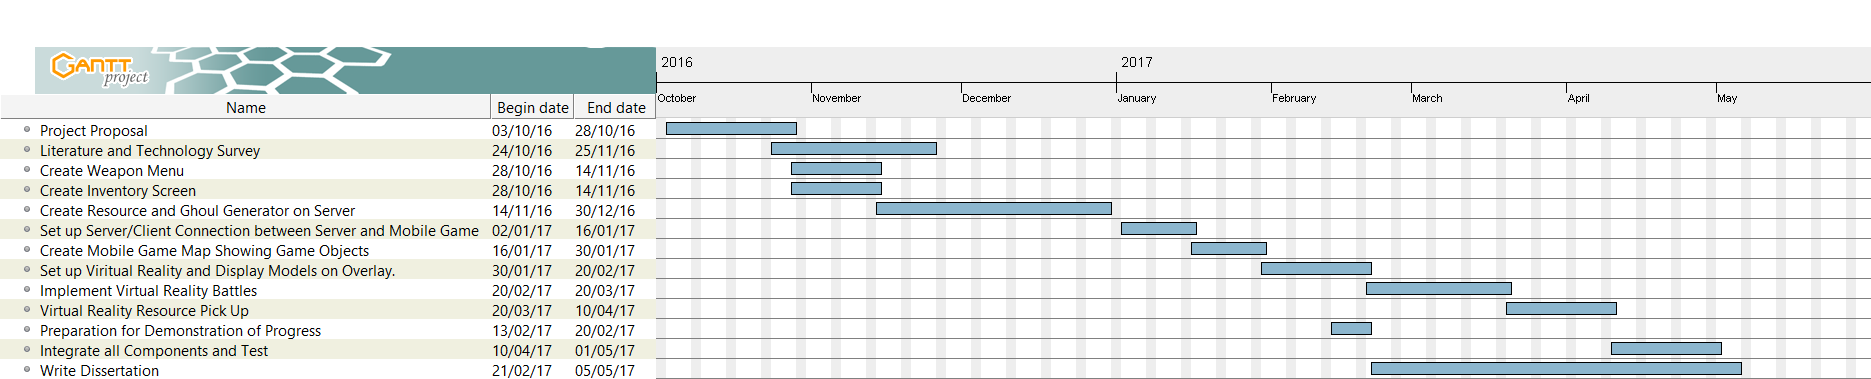
\includegraphics[width=150mm,height=60mm]{ProjectGanttChart.png}
			\caption{Ghantt Chart}
		\end{figure}
		
		\paragraph{Weeks 1 to 4:} I will write the project proposal. During this time I will not implement any of the game. The project proposal will help me understand what the game will look like. Therefore I want to start implementing the game after the project proposal.
		\newline
		\paragraph{Week 4 to 8:} Literature and Technology Survey: I will build upon the review of literature in the proposal by looking at the papers included in the proposal in more detail and find more papers that describe how to generate game objects directly or indirectly in the game.
		\newline
		\paragraph{Week 4 to 8:} I will start implementing Ghoul Hunter. I want to start with something that is relatively easy so I can find my feet using Unity. Therefore I am going to first implement the inventory screen and the weapon creation screen which are fairly simple screens. I will also learn how to use Unity's advanced features during this time including ARToolkit.
		\newline
		\paragraph{Week 8 to 13:} I will implement the server generation algorithms so that resources and ghouls can be generated. 
		\newline
		\paragraph{Week 13 to 15:} I will connect the mobile game to the server using a HTTP connection. 
		\newline
		\paragraph{Week 15 to 17:} I will implement the mobile game's game map. This should take too long as I would have already implemented Google maps on the Java server and the connection to the server should already be set up.
		\newline
		\paragraph{Week 20 to 21:} I will prepare the demonstration of progress where I will demonstrate the generation algorithms on the mobile game's game map. I will also show how the server and mobile game are connected. 
		\newline
		\paragraph{Week 17 to 27:} The augmented reality screen will be the hardest to implement due to it's complexity hence I have given it the most time. I will start with the ghoul battles and then move onto resource collection. 
		\newline
		\paragraph{Week 27 to  30:} I will integrate the whole game and make sure the game works in totality by doing user tests. Integration will include linking screens together. I want to finish a week before the final submission so that I can concentrate on the dissertation in the last week. 
		\paragraph{Week 19 to 31:}
		I will write the dissertation in parallel with the implementation of the game.
		
		\section{Appendix}
		\subsection{Requirements}
		This following requirements give a high level overview on what features the game needs to implement for both the server and the mobile game. \newline
		
		1. There will be four screens: a map screen, a weapon creation screen, an augmented reality screen and an inventory screen.
		
		\forceindent 1.1. The map screen will show a google map configured to the player's location.\newline
		\forceindent \forceindent 1.1.1. The map will have game objects drawn on top of it. \newline
		\forceindent \forceindent \forceindent 1.1.1.1. Near by resources will be drawn on the map.\newline
		\forceindent \forceindent \forceindent \forceindent 1.1.1.1.1. The type of the resource should be indicated.\newline
		\forceindent \forceindent \forceindent 1.1.1.2. Near by ghouls will be drawn on the map.\newline
		\forceindent \forceindent \forceindent \forceindent 1.1.1.2.1. The ghoul's level should be indicated.\newline
		\forceindent \forceindent 1.1.2. The position of the player will be drawn as a circle on the map.\newline
		
		\forceindent 1.2. The weapon creation screen will show the player's current weapon.\newline
		\forceindent \forceindent 1.2.1. The player should be able to swap out parts of their weapon with other parts which the player has created.\newline
		\forceindent \forceindent 1.2.2. Weapons should be split into three section:\newline
		\forceindent \forceindent \forceindent 1.2.2.1. The sharp end which could be filled with blades, maces and so on.\newline
		\forceindent \forceindent \forceindent 1.2.2.2. The poll which can be filled with a short poll for a short ranged weapon or a long poll for a long ranged weapon.\newline
		\forceindent \forceindent \forceindent 1.2.2.3. The handle which will be filled with a variety of different handle types. \newline
		
		\forceindent 1.3. The inventory screen should shown the players resources and their weapon parts in a grid.\newline
		\forceindent \forceindent 1.3.1. The player should be able to drag resources onto a box. \newline
		\forceindent \forceindent 1.3.1.1. The player should be able to then select a weapon part that can be created with those resources and create it such that they can use it later to create weapons. \newline
		
		\forceindent 1.4. The augmented reality screen should show two kinds of objects:
		\forceindent \forceindent 1.4.1. Ghouls which can be fought.\newline
		\forceindent \forceindent \forceindent 1.4.1.1. Fighting should consist of attacking and blocking.\newline
		\forceindent \forceindent \forceindent 1.4.1.2. The player aims attacks or blocks by pointing the sights at the ghoul. \newline
		\forceindent \forceindent \forceindent \forceindent 1.4.1.2.1. The player can then either press the attack button or the block button.\newline
		\forceindent \forceindent \forceindent 1.4.1.3. The ghoul will move so that the player will have to move the camera to the ghoul so it can block or attack the ghoul.\newline
		\forceindent \forceindent \forceindent \forceindent 1.4.1.3.1. An arrow will appear showing which direction the ghoul is so that the player knows where to turn the phone.\newline
		\forceindent \forceindent \forceindent \forceindent 1.4.1.3.2. The ghoul should be able to move rotationally around the player or increase it's radius from the player.\newline
		\forceindent \forceindent \forceindent \forceindent \forceindent 1.4.1.3.2.1. A ghoul must not move more than it's own range from the player. \newline
		\forceindent \forceindent \forceindent  1.4.1.4. The ghoul has to appear as a 3d model on the camera image if the player is facing the ghoul.\newline
		\forceindent \forceindent \forceindent 1.4.1.5. If the player wins the fight they can collect a diamond.
		\forceindent \forceindent \forceindent \forceindent 1.4.1.5.1. The diamond is added to the players inventory and can be used as a resource to improve weapons.\newline
		\forceindent \forceindent \forceindent 1.4.1.6. If the player loses a fight the ghoul disappears and the player gets nothing.\newline
		\forceindent \forceindent \forceindent 1.4.1.7. The higher the ghoul's level the more difficult it is to destroy.\newline
		\forceindent \forceindent \forceindent \forceindent 1.4.1.7.1. High level ghouls will only be possible to kill by players who have good weapons and are skilled at fighting ghouls.\newline
		\forceindent \forceindent \forceindent 1.4.1.8. The better the player's weapon the more damage they will be able to inflict upon the ghoul and the better they will block.\newline
		\forceindent \forceindent \forceindent \forceindent 1.4.1.8.1. Different weapons will have different strengths.\newline
		\forceindent \forceindent \forceindent \forceindent \forceindent 1.4.1.8.1.1. Weapons will long polls will have longer range than those with short polls.\newline
		\forceindent \forceindent \forceindent \forceindent \forceindent 1.4.1.8.1.2. Weapons with blades will be more accurate meaning that the player's sight will be bigger but will inflict less damage upon the ghoul.\newline
		\forceindent \forceindent \forceindent \forceindent \forceindent 1.4.1.8.1.3. Weapons with maces or spiked balls will be less accurate meaning that the player's slight will be smaller but will inflict more damage upon the ghoul. \newline
		\forceindent \forceindent 1.4.2. Resources which can be collected. \newline
		\forceindent \forceindent \forceindent 1.4.2.1. The player must be able to aim the screen's sights on the resource and collect it by pressing a collect button. \newline
		\forceindent \forceindent \forceindent 1.4.2.2. If the resource is out of the sights then an arrow should appear showing which angle the phone needs to be moved.\newline
		\forceindent \forceindent \forceindent 1.4.2.3. The resources should be drawn on the camera image with a 3d model. \newline
		\forceindent \forceindent 1.4.3. The augmented reality screen should only show a game object if it is close to the player.\newline
		
		2.	The mobile game should be able to connect to a server that give the mobile game information about what is around the player.\newline
		\forceindent 2.1.	Server should only send information on request.\newline
		
		\forceindent 2.2 Sever should generate game object in a balance fashion.\newline
		\forceindent \forceindent 2.2.1. Server should generate resources.\newline
		\forceindent \forceindent \forceindent 2.2.1.1. Using google maps the server should generate resources only in certain areas.\newline
		\forceindent \forceindent \forceindent \forceindent 2.2.1.1.1. Wood in green areas.\newline
		\forceindent \forceindent \forceindent \forceindent 2.2.1.1.2. Stone on roads.\newline
		\forceindent \forceindent \forceindent \forceindent 2.2.1.1.3. Iron in buildings.\newline
		\forceindent \forceindent 2.2.2. Server should generate ghouls.\newline
		\forceindent \forceindent \forceindent 2.2.2.1. Ghouls should be evenly distributed so that ghouls of a variety of levels are around the same area.\newline
		\forceindent \forceindent \forceindent 2.2.2.2. The higher the ghoul's level the less likely it will generate. \newline
		\forceindent \forceindent 2.2.3. The quantity of ghouls and resources should be based on the population density of an area.\newline
		\forceindent \forceindent \forceindent 2.2.3.1. Any area should have enough resources and ghouls to satisfy the number of player likely to be playing there. \newline
		\forceindent \forceindent 2.2.4. Resources should be diversely distributed for example some areas buildings should produce less iron than other but the adjacent green areas produce more wood. This is to provide an incentive for players to move to other areas. \newline
		
		\forceindent2.3. When the player fights a ghoul it should disappear from the map regardless of the result of the battle.\newline
		
\bibliography{proposalBib}
\end{document}